%% Adaptado de 
%% http://www.ctan.org/tex-archive/macros/latex/contrib/IEEEtran/
%% Traduzido para o congresso de IC da USP
%%*****************************************************************************
% Não modificar

\documentclass[twoside,conference,a4paper]{IEEEtran}
\makeatletter
\def\endthebibliography{%
  \def\@noitemerr{\@latex@warning{Empty `thebibliography' environment}}%
  \endlist
}
\makeatother


%******************************************************************************
% Não modificar
\usepackage{IEEEtsup} % Definições complementares e modificações.
\usepackage[utf8x]{inputenc} % Disponibiliza acentos.
\usepackage[english,brazil]{babel}
%% Disponibiliza Inglês e Português do Brasil.
\usepackage{latexsym,amsfonts,amssymb} % Disponibiliza fontes adicionais.
\usepackage{theorem} 
\usepackage[cmex10]{amsmath} % Pacote matemático básico 
\usepackage{url} 
%\usepackage[portuges,brazil,english]{babel}
\usepackage{graphicx}
\usepackage{amsmath}
\usepackage{amssymb}
\usepackage{color}
\usepackage[pagebackref=true,breaklinks=true,colorlinks,bookmarks=false]{hyperref}
\usepackage[tight,footnotesize]{subfigure} 
\usepackage[noadjust]{cite} % Disponibiliza melhorias em citações.
\usepackage[]{algorithm2e}
\usepackage{dirtytalk}
\usepackage{lscape}

%%*****************************************************************************

\begin{document}
    \selectlanguage{english}
    \renewcommand{\IEEEkeywordsname}{Palavras-chave}
    \definecolor{black}{gray}{0}    
    %%*****************************************************************************
    
    \urlstyle{tt}
    % Indicar o nome do autor e o curso/nível (grad-mestrado-doutorado-especial)
    \title{Final Project - MC907 A}
    \author{%
        \IEEEauthorblockN{Luiz Eduardo Cartolano,\IEEEauthorrefmark{1}}
        \IEEEauthorblockA{\IEEEauthorrefmark{1}
                           Computer Engineer - Undergraduate \\
                           \IEEEauthorrefmark{1}E-mail: l183012@students.ic.unicamp.br }
    }
    
    %%*****************************************************************************
    
    \maketitle
    
    %%*****************************************************************************
    % Resumo do trabalho
\begin{abstract}
    In robotics and computer vision, visual odometry is the process of determining the position and orientation of a robot by analyzing the associated camera images. It has been used in a wide variety of robotic applications, such as on the Mars Exploration Rovers. The classical approaches for solve the VO problems are usually based on the kinematics of the robot, so they can be easily induced to fail when either the motion of the robot or the environment are too challenging. In this way, novel VO methods use deep neural networks or attention models to improve or even replace the entire algorithm pipeline. In this project, we aim to brief introduce both algorithms and given sample results of the frameworks. Some obtained results are show in Figures \ref{fig:train150}, \ref{fig:seq2}, \ref{fig:seq4} and \ref{fig:seq5}. A video with the model results is available at \url{https://biteable.com/watch/deepvo-2406592}.
\end{abstract}
    
    % Indique três palavras-chave que descrevem o trabalho
    \begin{IEEEkeywords}
        Deep Learning - Visual Odometry - Robotics
    \end{IEEEkeywords}
    
    %%*****************************************************************************
    \section{Introduction}
        Visual Odometry (VO) is one of the most essencial techniques for pose estimation and robot localization now a days. The classical approach for VO systems is shown in Figure \ref{fig:1}, which typically consists of camera calibration, feature detection, feature matching, outlier rejection, scale estimation and local optimisation, has been developed and broadly recognised as a golden rule to follow. Altough the state-of-the-art algorithms based on this pipeline have shown excellent performance, they are usually hard-coded, where each module of the pipeline is adapted to the hardware in order to achieve an amazing performance. 
        
        In parallel, in the last years, Deep Learning (DL) \cite{lecun2015deep}, has been dominating many computer vision tasks with spectacular results. Unfortunately, for the VO problem this has not fully arrived yet, walking in short steps. In this work, we are going to present some new approachs that uses DL for the VO problem. Most of them consist at a Deep Recurrent Convolutional Neural Networks to solve the problem. One of the first articles that addresses the solution is shown at \cite{wang2017deepvo} and a pipeline is shown at Figure \ref{fig:2}.
        
        Another approach that has been gaining attention, is the use of a visual saliency map in order to increase the performance of the state-of-the-art algorithms. The concept is quite simple, as we are going to futher explain, humans perform the task of mapping very differently from how it has been usually done at the classical approaches at robotics \cite{liang2019salientdso}.
        
        For this work, we aim to focus our efforts at the Deep Learning approach. This paper is organized as follows: Section \ref{sec:trabalho-proposto}  presents how the paper was organized in order to solve the problem. Section \ref{sec:metodos} describes the tests done and the methodologies covered. The results and analysis are presented in Section \ref{sec:res-dic} and finally, the conclusions at Section \ref{sec:conclusao}.
    \section{Proposed Work}\label{sec:trabalho-proposto}
    
    The proposed work, which can be seen in more detail in \citeonline{enun}, calls for the implementation of a project to solve a classical robotic problem. To explain the work in more detail, the next subsections will cover the problem and the tools used to solve it.
    
    \subsection{Problem}
        In robotics and computer vision, visual odometry is the process of determining the position and orientation of a robot by analyzing the associated camera images. This work aims to implement a end-to-end Deep Learning technique to preview the robot position at the enviroment.
        
    \subsection{Tools}\label{sec:org-proj}
        In order to carry out the proposed implementations it was used as programming language the $3.7$ version of Python. In conjunction with it, the Jupyter Notebook platform was used, since with it's easier to track the results of the applied algorithms and also because it allows the execution of specific pieces of code, which ensures greater flexibility in using the various algorithms used.
    \section{Materials and methods} \label{sec:metodos}
    In this section we will explain in more detail the problem modeling, ie the machine learning techniques implemented in the project and how they were specified.
    
    \subsection{Related Work - Deep VO}
        The paper \cite{wang2017deepvo} presents a novel end-to-end framework for monocular VO by using deep Recurrent Convolutional Neural Networks (RCNNs) \cite{liang2015recurrent}. Since it is trained and deployed in an end-to-end manner, it infers poses directly from a sequence of raw RGB images (videos) without adopting any module in the conventional VO pipeline. Based on the RCNNs, it not only automatically learns effective feature representation for the VO problem through Convolutional Neural Networks, but also implicitly models sequential dynamics and relations using deep Recurrent Neural Networks. The framework has been tested under the Kitti Dataset \footnote{\url{http://www.cvlibs.net/datasets/kitti/eval_odometry.php}}, showing great results.
        
        The model is mainly composed of CNN based feature extraction, as previous presented in \cite{chen2016deep}, and RNN based sequential modelling, as shown in \cite{chung2015recurrent}. The architecture of the proposed VO system is shown in Figure \ref{fig:8}, it takes a monocular image sequence as input. Two consecutive images are stacked together to form a tensor for the deep RCNN to learn how to extract motion information and estimate poses. The VO system develops over time and estimates new poses as images are captured. 
        
        The image feature extraction of is done by a CNN, which configuration is shown at Figure \ref{fig:9}. The CNN takes raw RGB images instead of pre-processed counterparts, such as optical flow or depth images, as input because the network is trained to learn an efficient feature representation with reduced dimensionality for the VO.
        
        Following the CNN, a deep RNN is designed to conduct sequential learning, i.e., to model dynamics and relations among a sequence of CNN features. Since the RNN is capable of modelling dependencies in a sequence, it is well suited to the VO problem which involves temporal model (motion model) and sequential data (image sequence). 
        
        To learn the hyperparameters $\theta$ of the DNNs, the Euclidean distance between the ground truth pose ($p_k$ ,$\varphi_k$) at time $k$ and its estimated one ($\text{\^{p}}_k$ ,$\hat{\varphi_k}$) is minimised. The loss function is composed of Mean Square Error (MSE) of all positions p and orientations :
        \begin{equation}
            \theta^* = \underset{\theta}{\mathrm{argmin}} \frac{1}{N} \sum_{i=1}^{N}\sum_{k=1}^{t} \left\| \hat{p_k} - p_k \right\|^{2}_2 + k \cdot \left\| \hat{\varphi_k} - \varphi_k \right\|^{2}_2
            \label{eq:MSE}
        \end{equation}
        
         In Figure \ref{fig:10}, the losses results of the models are given for both training and validate datasets. As shown in the fig., the loss significantly reduces with time, and, once the training and validation losses shown a similar behavior we can also say that is free of overfiting, so, the model is well-fit.
         
         The Figures \ref{fig:11} and \ref{fig:12} show us the obtained maps for the framework for both training and test datasets. As we can see in the figures, the obtained odometry from the system is very close to the ground truth position, showing how great the system performs. The system is analysed according to the KITTI VO/SLAM evaluation metrics, i.e., averaged Root Mean Square Errors (RMSEs) of the translational and rotational errors for all subsequences of lengths ranging. The average RMSEs of the estimated VO are given in Figure \ref{fig:13}. Al- though the result of the DeepVO is worst than that of the stereo VISO2 (VISO2\_S), it is consistently better than the monocular VISO2 (VISO2\_M).
         
         The paper presents a novel end-to-end monocular VO algorithm based on Deep Learning, that does not depend on any module in the conventional VO algorithms (even camera calibration) for pose estimation and it is trained in an end-to-end manner, there is no need to carefully tune the parameters of the VO system. Based on the KITTI VO benchmark, it is verified that it can produce accurate VO results with precise scales and work well in completely new scenarios.
         
         For this project, we aim to reproduce the paper approach using images and poses obtained at the AirSim, an open source simulator for autonomous vehicles built on Unreal Engine/Unity, from Microsoft AI\&Research \footnote{\label{ref:note1}\url{https://github.com/microsoft/AirSim}}.
         
    \subsection{Project Dataset}
        \subsubsection{Data Collection}
            In order to create our own \emph{dataset} to perform the article model we had use the Microsoft AirSim Simulator to generate both images and poses.
            
            Six sequences were generated under three different scenarios: Neighborhood(Figure \ref{fig:neig}), Africa (Figure \ref{fig:africa}) and LandscapeMountains(Figure \ref{fig:mountain}). 
            
            The simulator were used at the \emph{ComputerVision} mode and the cameras controlled via keyboard. Each sequence has around four hundred pictures, making a total of around two thousand images for the training set.
        
        \subsubsection{Images Data Prerocessing}
            The first stage of image preprocessing was eliminate all failed pictures given by the simulator, excluding them from both pictures and pose lists.
            
            After that, as we read the images we convert them to grayscale and normalize their pixels values, in a range that goes from -0.5 to 0.5 in order to be able to use the pretrained weight of FlowNet, all of it were done using the OpenCV library.
            
            At least, we concatenated the pictures two by two, once that the two images will going to work as input for our Neural Network.
            
        \subsubsection{Poses Data Preprocessing}
            The AirSim recording mode, as we further explain, give us a text file with the following informations for each image: timestamp, x\_position, y\_position, z\_position, quaternions\_x, quaternions\_y, quaternions\_z, quaternions\_w and a filename of the image associated to that pose.
            
            As explained in \citeonline{quat_angle}, a quaternion is a four-element vector that can be used to encode any rotation in a 3D coordinate system.  Technically, a quaternion is composed of one real element and three complex elements, and it can be used for much more than rotations. For our work, we need the angles to be at an Euler representation. Euler angles provide a way to represent the 3D orientation of an object using a combination of three rotations about different axes.
            
            In order to transform the given angles to an Euler representaion we need to use the following equations:
            
            \begin{equation}
                \phi = arctan(\frac{2(ab+cd)}{a^2 - b^2 - c^2 + d^2})
            \end{equation}
            \begin{equation}
                \theta = -arcsin(2(bd-ac))
            \end{equation}
            \begin{equation}
                \Psi = arctan(\frac{2(ad+bc)}{a^2 + b^2 - c^2 - d^2}
            \end{equation}
            
            This can be easily done in \emph{Python} using the \emph{Scipy} \footnote{\url{https://docs.scipy.org/doc/scipy-1.2.1/reference/generated/scipy.spatial.transform.Rotation.html}} library.
            
            Another thing we had to do in order to process the information was make the first pose our start point, so we subtract all the other poses from the first one value. In addition, in addition we subtract all the poses, with the except of the firts, from the previous pose value, so, the network has to predict only the dislocate between two images.
            
    \subsection{Deep VO Implementation}
        In order to simulate Wang's\cite{wang2017deepvo} paper for our dataset, we implemented the same RCNN model showed at Figure \ref{fig:2}.
        
        For implementing the model we used the PyTorch \footnote{\url{https://pytorch.org/}} library. All the convolutionals layers has a \emph{Conv2d} structure, followed by a \emph{BatchNorm2d} (batch normalization), and then a \emph{LeakyReLU} function (a Rectified Linear Activation Function) and in the end, a \emph{Dropout}.
        
        A convolution is the simple application of a filter to an input that results in an activation, the batch normalization reduces the amount by what the hidden unit values shift around (covariance shift). The activation function is responsible for transforming the summed weighted input from the node into the activation of the node or output for that input. And in the dropout stage, at each training stage, individual nodes are either dropped out of the net with probability 1-p or kept with probability p, so that a reduced network is left; incoming and outgoing edges to a dropped-out node are also removed.
        
        For the CNN part we tested two different configurations, which results will be further commented. We first fitted the model without any previous information and, in a second stage, we loaded pretrained weight of FlowNet network \footnote{\url{https://towardsdatascience.com/a-brief-review-of-flownet-dca6bd574de0}}.
        
        For the RNN part of the network, we had two \emph{LSTM} layers followed by a linear output, that receives 100 features as input and outputed 6 features (our pose). The Long Short-Term Memory (LSTM) networks are a modified version of recurrent neural networks, which makes it easier to remember past data in memory.
        
        To define the loss function we used the Mean Square Error, same as Wang's paper and which equations is defined at Equation \ref{eq:MSE}. The used optimizer was the Adagrad, an algorithm for gradient-based optimization that does just this: It adapts the learning rate to the parameters, performing smaller updates (i.e. low learning rates) for parameters associated with frequently occurring features, and larger updates (i.e. high learning rates) for parameters associated with infrequent features.        
    \section{Results and Discussion} \label{sec:res-dic}
    In this section we will first present all the results obtained during the implementation of the implemented solution, including tables and graphs generated. Once introduced, they will be discussed and compared.
    
    \subsection{Results} \label{sec:resultados}
        At Figures \ref{fig:train90} and \ref{fig:train150} we are able to see the training losses of the two different experiences made with the implemented neural network. The Figure \ref{fig:train90} shows the training loss for 90 epochs when we didn't use the pretrained weigths of FlowNet, while the Figure \ref{fig:train150}, shows the results for 150 epochs using the pretrained weigths of FlowNet. These results, as we are going to further discuss were a lot worst than the obtained by \cite{wang2017deepvo}. 
        
        After fit the model we work on validate the obtained weights on a different sequence that were designated as a test dataset. The first measure we did were measure the accuracy of the system. The accuracy were calculated by the follow equation:
        \begin{equation}
            acc = \frac{1}{N} \sum_{i=1}^{N}\sum_{k=1}^{t} \left\| \hat{p_k} - p_k \right\|^{2}_2 + \left\| \hat{\varphi_k} - \varphi_k \right\|^{2}_2
        \end{equation}
        And we obtained an accuracy of \emph{54.70\%}. We also analyse the individual erros for position (x,y,z) and orientation, obtaining results of \emph{9.81\%} and \emph{58.84\%}.
        
        Lastly, we can present as a result the odometry provided by our system ploted with the original position, the ground truth one. Figures \ref{fig:seq2}, \ref{fig:seq4} and \ref{fig:seq5} shows that results. The blue line on the figures show the ground truth position given by the simulator and the green line the odometry given by our model.
        
    \subsection{Discussion} \label{sec:discussao}
        Firts we are going to compare the training losses obtained in our experiment for two different scenarios under the same dataset. Comparing Figures \ref{fig:train90} and \ref{fig:train150}, it's possible to realize that the pretrained weigths of FlowNet weren't a big differential to fitting the model. Both of the experiments shows signals of over-fit, because the validation loss don't reduce as the same ratio of training loss. Actually, the validation still the same all over both experiments. The main reason of that results are, very likely, the number of images and poses used on training, that were far bellow the necessary.
        
        Since we have an experiment that we were looking for to reproduce, we can also compare our results with them. If we look for Figure \ref{fig:10}, we realized that Wang's model were a lot better fitted and different of ours didn’t show any signal of over-fit. A main difference in both experiments is the number of images used for training, at \cite{wang2017deepvo} they used almost 7 thousand images from the Kitti dataset, while we used among 2 thousand images, which reinforce our previous idea that the main reason of over-fit were the number of images used for fit the model.
        
        Analysing the accuracy results lead us to a very interesting perspective about the system performance, that is well better when predict angles deslocation than position. The most likely reason for that is on how images were collected in the simulator, the deslocation between to images is very abrupt.
        
        Lastly is time to analyse the most visual of all results we obtained, the images comparing the ground truth and the odometry. If we look for Figure \ref{fig:seq2} it's possible to see that the ground truth has a lot of abrupt changes on both axis directions and this changes are not identified by the model. Figure \ref{fig:seq4}, on the other hand, has a much smoother trajectory, what makes the odometry a lot more accurate, but still not able to manage a sharp turn. Figure \ref{fig:seq5} has the smoothest of all the trajectories, even on that the model were far away to show a good preview.
        
        The same way compared the training losses of our project with Wang's, we can also compare our odometry with the one obtained by Wang in \cite{wang2017deepvo} (Figure \ref{fig:11}), even showing some big differences between the ground truth and the odometry the system is much more accurate than the one we obtained. There are few possible reasons for that. First, the fact that our model had over-fit. Second, the images fom the Kitti dataset our way more friendly than the ones from the simulator, since they are obtained by an autonomous car which made it smoother, with a constant velocity and also, the images are rectified (Image rectification is a transformation process used to project images onto a common image plane).
    \section{Conclusions} \label{sec:conclusao}
    In general, the work did not show great results. But, it definitely was great for first experiment with the subject. Also, it was amazing to introduce with the application of machine learning techniques for the visual odometry problem.
    
    Some positive points we can extract from this work is the fact that the using of Deep Learning techniques are plausible to the VO problem, and also, they showed that the simulator images are a good path to make a dataset for the problem.
    
    Weaknesses of the work, which need to be improved in future iterations, are the number of images in the dataset, also some improvements on the neural network, in order to ensure a better fit to the model. Also, we could improve system's effectiveness is to add some kind of SLAM \cite{lim2014real} or a salient model to preprocessing the images.
        
    %******************************************************************************
    % Referências - Definidas no arquivo Relatorio.bib
     +-------------+
    
    \bibliographystyle{IEEEtran}
    \bibliography{relatorio}
    %******************************************************************************
    
    \newpage
    \section*{Attachments}
    % \begin{equation}
    %     distancia = \sqrt{ (x_{goal} - x_{state})^2 + (y_{goal} - y_{state})^2 }
    %     \label{eq:distancia-dois-pontos}
    % \end{equation}
    
    % \begin{figure}[h!]
    %     \centering
    %     \includegraphics[width=0.5\hsize]{figuras/cnn.png}
    %     \caption{Estrutura da Rede Convolucional.}
    %     \label{fig:cnn-arq}
    % \end{figure}
    
    \begin{figure}[h]
        \centering
        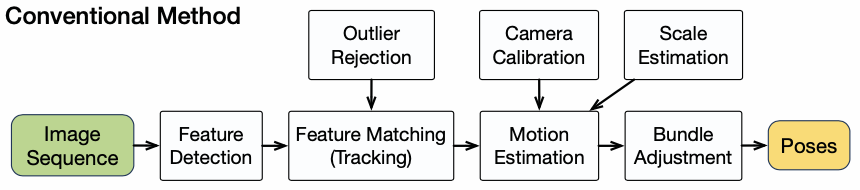
\includegraphics[width=0.75\columnwidth]{figuras/figura1.png}
        \caption{Classical pipeline for Visual Odometry.}
        \label{fig:1}
    \end{figure}

    \begin{figure}[h]
        \centering
        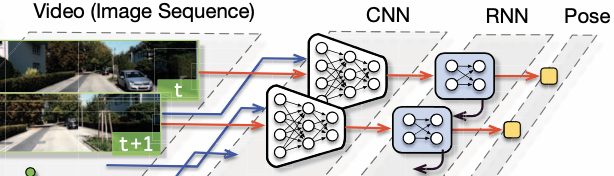
\includegraphics[width=0.75\columnwidth]{figuras/figura2.png}
        \caption{DeepVO pipeline for Visual Odometry.}
        \label{fig:2}
    \end{figure}
    
    \begin{figure}[h]
        \centering
        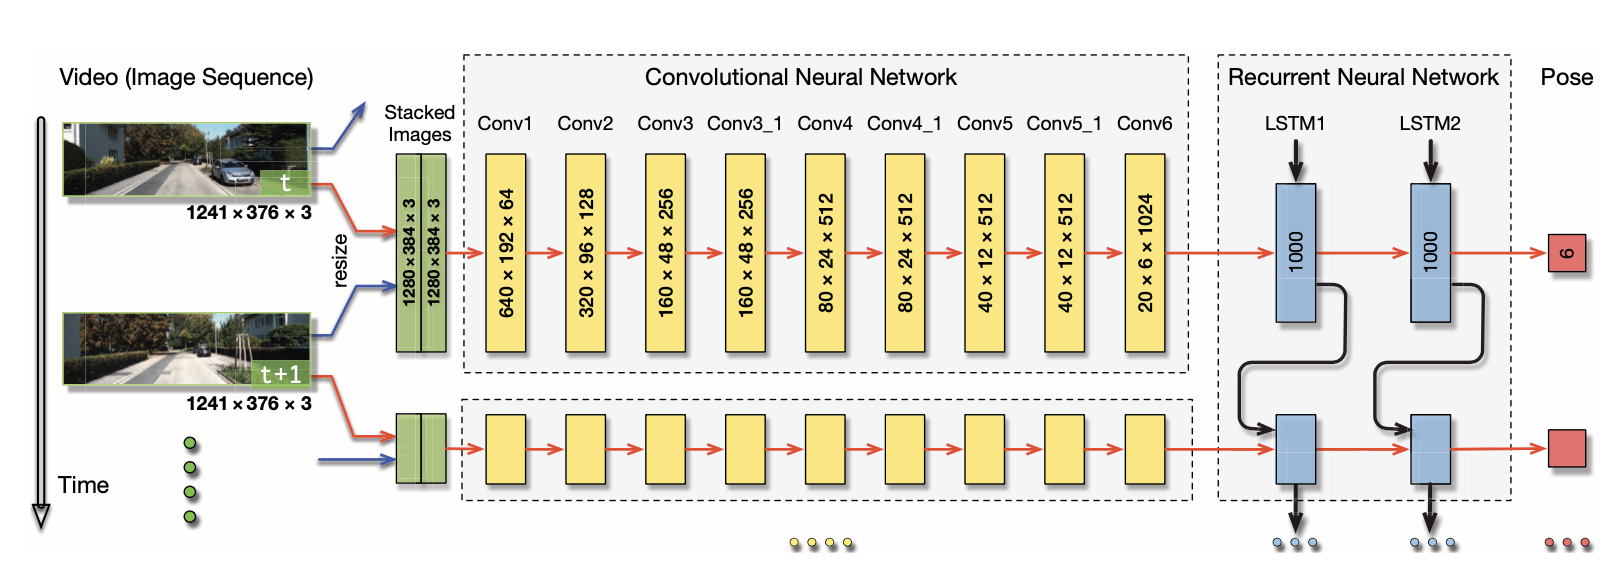
\includegraphics[width=0.65\columnwidth]{figuras/figura8.png}
        \caption{Architecture of the RCNN monocular VO system.}
        \label{fig:8}
    \end{figure}        
    
    \begin{figure}[h]
        \centering
        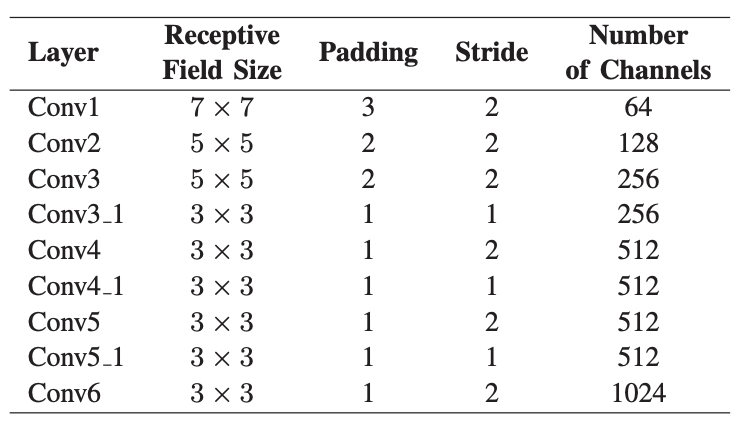
\includegraphics[width=0.65\columnwidth]{figuras/figura9.png}
        \caption{Configuration of the CNN for monocular VO system.}
        \label{fig:9}
    \end{figure}
    
    \begin{figure}[h]
        \centering
        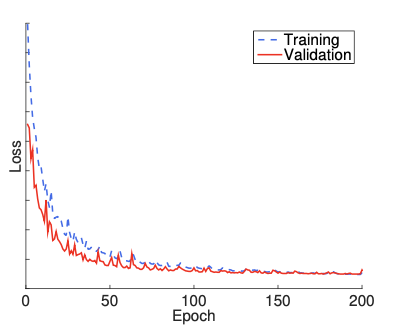
\includegraphics[width=0.65\columnwidth]{figuras/figura10.png}
        \caption{Training losses for the monocular VO system for the Wang paper.}
        \label{fig:10}
    \end{figure}
    
    \begin{figure}[h]
        \centering
        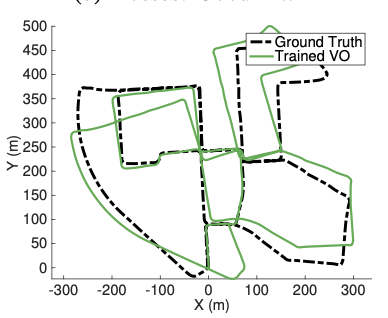
\includegraphics[width=0.65\columnwidth]{figuras/figura11.png}
        \caption{Obtained map for the monocular VO system under the training dataset for the Wang paper.}
        \label{fig:11}
    \end{figure}        

    \begin{figure}[h]
        \centering
        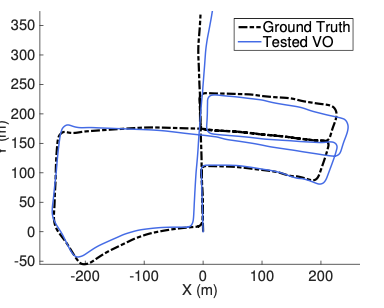
\includegraphics[width=0.65\columnwidth]{figuras/figura12.png}
        \caption{Obtained map for the monocular VO system under the test dataset for the Wang paper.}
        \label{fig:12}
    \end{figure}

    \begin{figure}[h]
        \centering
        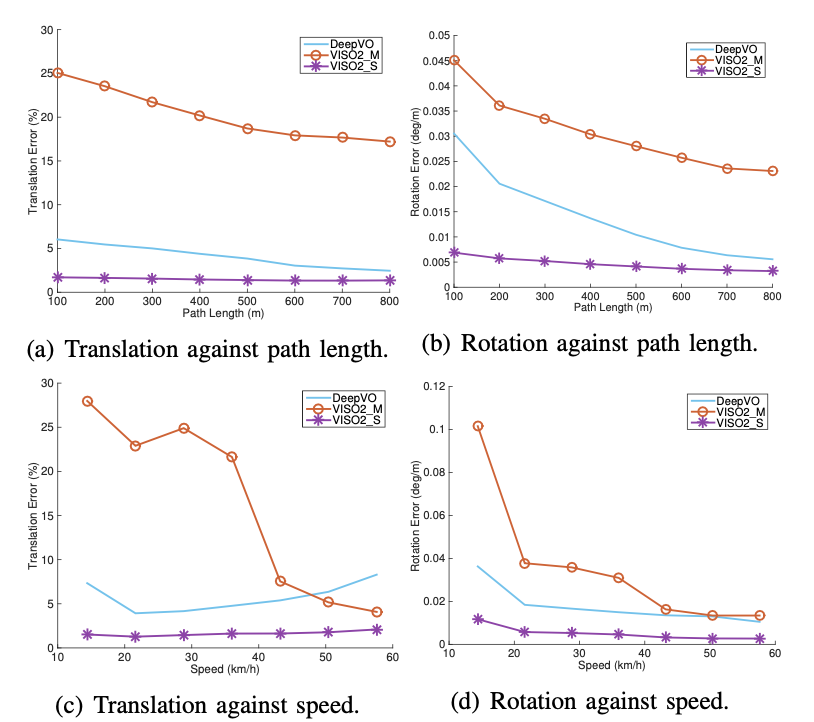
\includegraphics[width=0.65\columnwidth]{figuras/figura13.png}
        \caption{Average errors on translation and rotation against different path lengths and speeds for the Wang paper.}
        \label{fig:13}
    \end{figure}
    
    \begin{figure}[h]
        \centering
        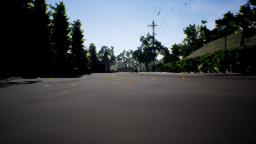
\includegraphics[width=0.65\columnwidth]{figuras/neig.png}
        \caption{Example of image obtained at the Neighbourhood scene from AirSim.}
        \label{fig:neig}
    \end{figure}
    
    \begin{figure}[h]
        \centering
        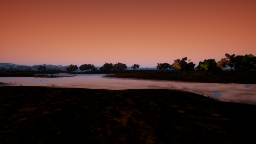
\includegraphics[width=0.65\columnwidth]{figuras/africa.png}
        \caption{Example of image obtained at the Africa scene from AirSim.}
        \label{fig:africa}
    \end{figure}
    
    \begin{figure}[h]
        \centering
        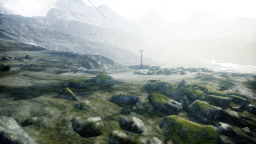
\includegraphics[width=0.65\columnwidth]{figuras/mountains.png}
        \caption{Example of image obtained at the LandscapeMountains scene from AirSim.}
        \label{fig:mountain}
    \end{figure}
    
    \begin{figure}[h]
        \centering
        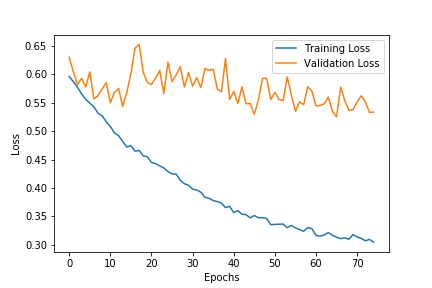
\includegraphics[width=0.65\columnwidth]{figuras/train_batch_dropout_90.png}
        \caption{Training losses without the weights of FlowNet.}
        \label{fig:train90}
    \end{figure}
    
    \begin{figure}[h]
        \centering
        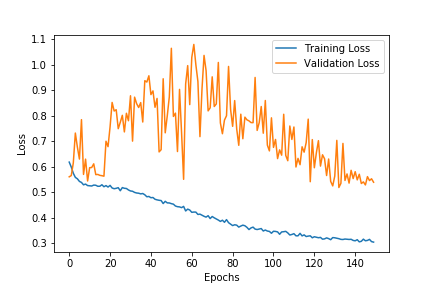
\includegraphics[width=0.65\columnwidth]{figuras/train_batch_dropout_150.png}
        \caption{Training losses with the weights of FlowNet.}
        \label{fig:train150}
    \end{figure}
    
    \begin{figure}[h]
        \centering
        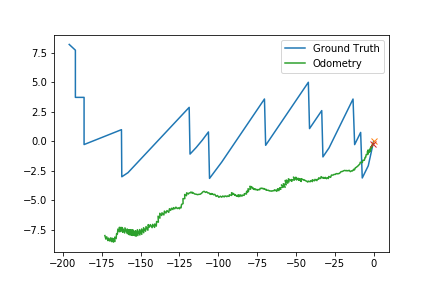
\includegraphics[width=0.65\columnwidth]{figuras/testeSeq2.png}
        \caption{Comparison between the ground truth position and the odometry provided by the system for the first test sequence.}
        \label{fig:seq2}
    \end{figure}
    
    \begin{figure}[h]
        \centering
        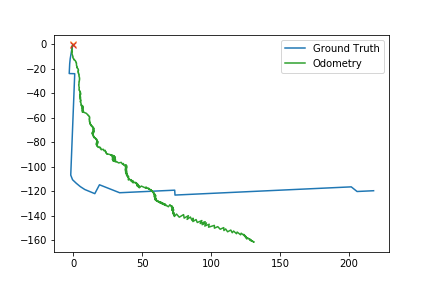
\includegraphics[width=0.65\columnwidth]{figuras/testeSeq4.png}
        \caption{Comparison between the ground truth position and the odometry provided by the system for the second test sequence.}
        \label{fig:seq4}
    \end{figure}
    
    \begin{figure}[h]
        \centering
        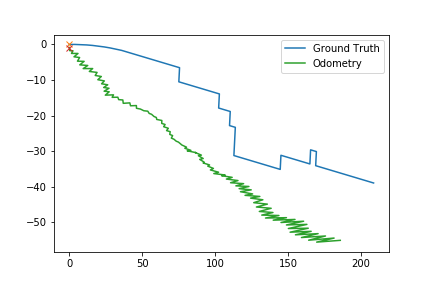
\includegraphics[width=0.65\columnwidth]{figuras/testeSeq5.png}
        \caption{Comparison between the ground truth position and the odometry provided by the system for the third test sequence.}
        \label{fig:seq5}
    \end{figure}

\end{document}
